\chapter{Literature}
\section{Quinachridone (QA)}

The examined adsorbate \acf{QA} is a high symmetric, prochiral organic molecule with the full IUPAC name 5,12-dihydro-quino[2,3-\textit{b}]acridine-7,14-dione and the sum formula \ce{C20H12N2O2}. Organic crystals exhibit a color which can range from red to violet.\autocite{ChemicalBook2025,ChemSpider2025}

\ac{QA} is most prominently recognized as the parent structure of a group of pigments, most notably Pigment Violet 19 (C.I. 73900). This particular pigment is extensively utilized in industrial applications due to its remarkable color properties and stability.\autocite{ChemicalBook2025,ChemSpider2025} The molecular structure of \ac{QA} is shown in \autoref{fig:QA}.

\begin{figure}[H]
	\centering
	\begin{subfigure}[b]{0.48\linewidth}
		\centering
		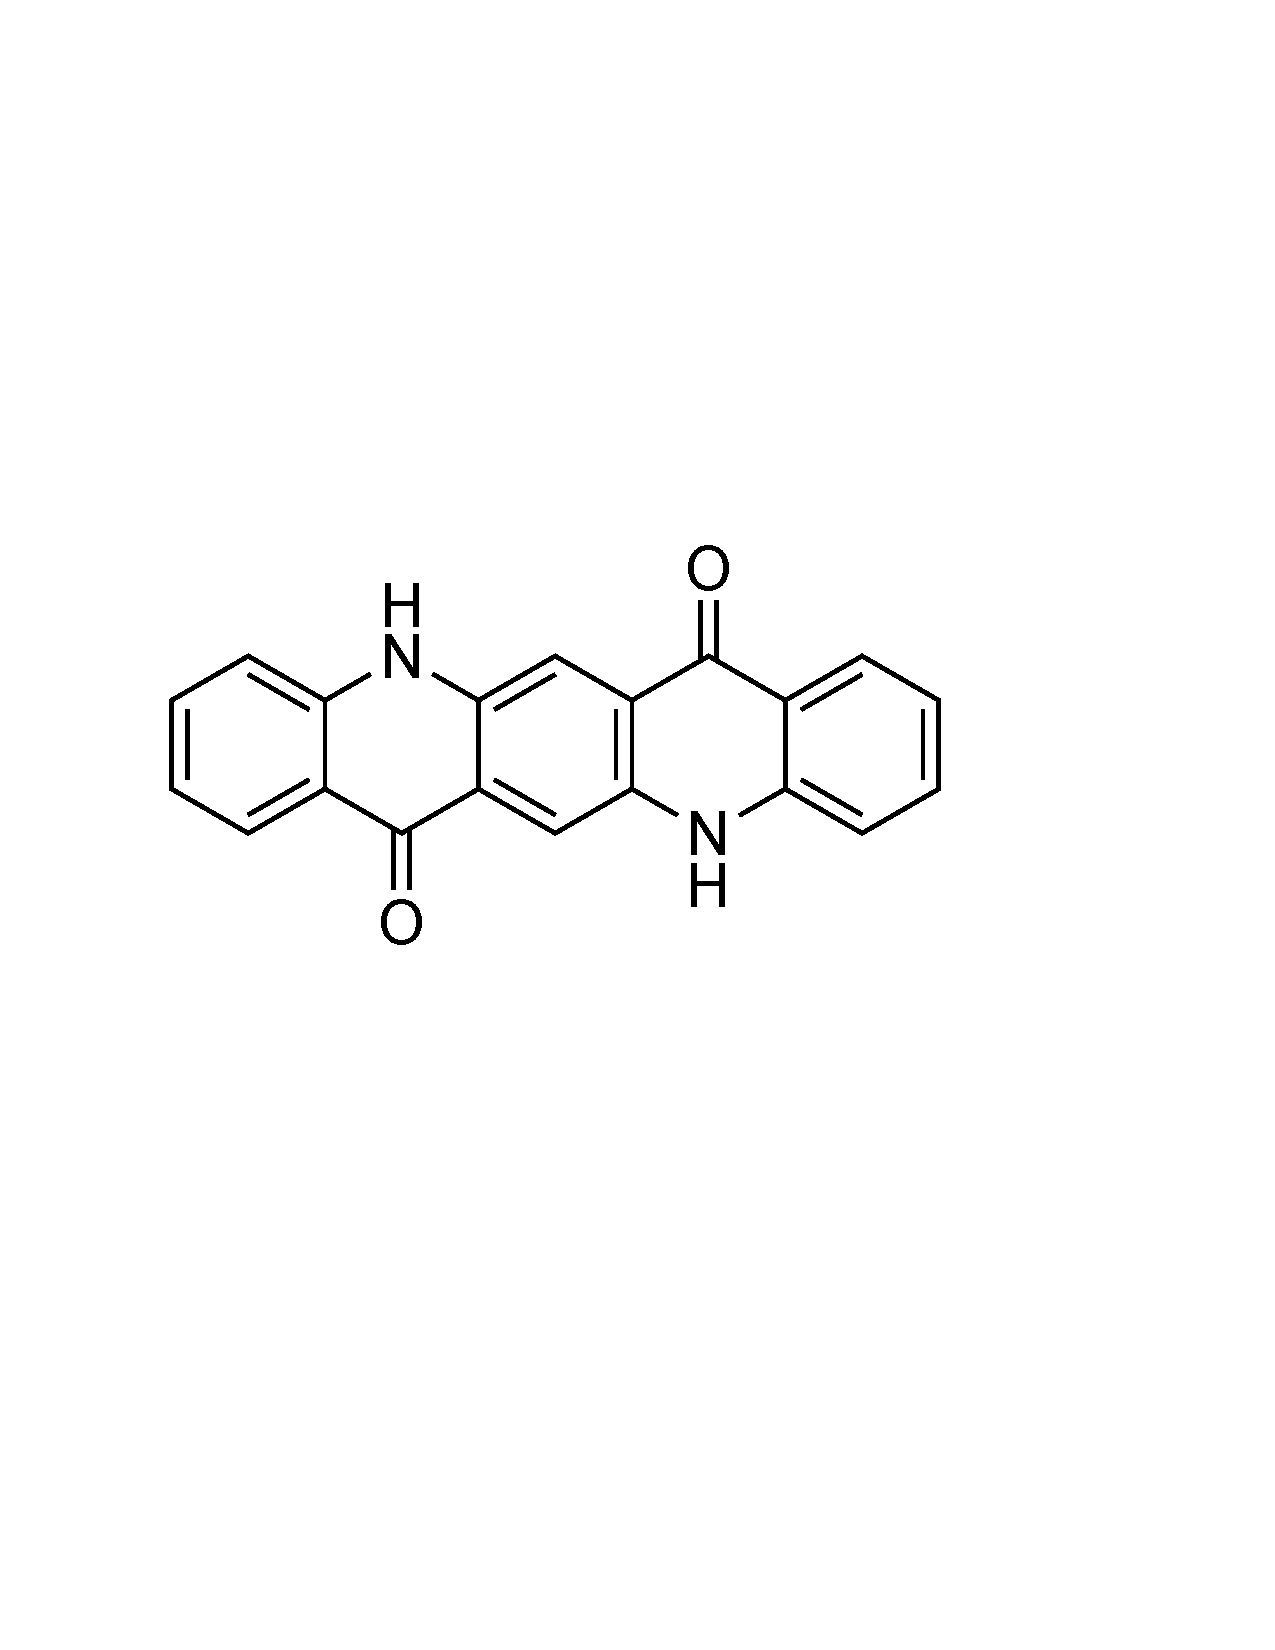
\includegraphics[width=\linewidth]{images/QA.pdf}
		\caption{Skeletal structure}
	\end{subfigure}
	\hfill
	\begin{subfigure}[b]{0.48\linewidth}
		\centering
		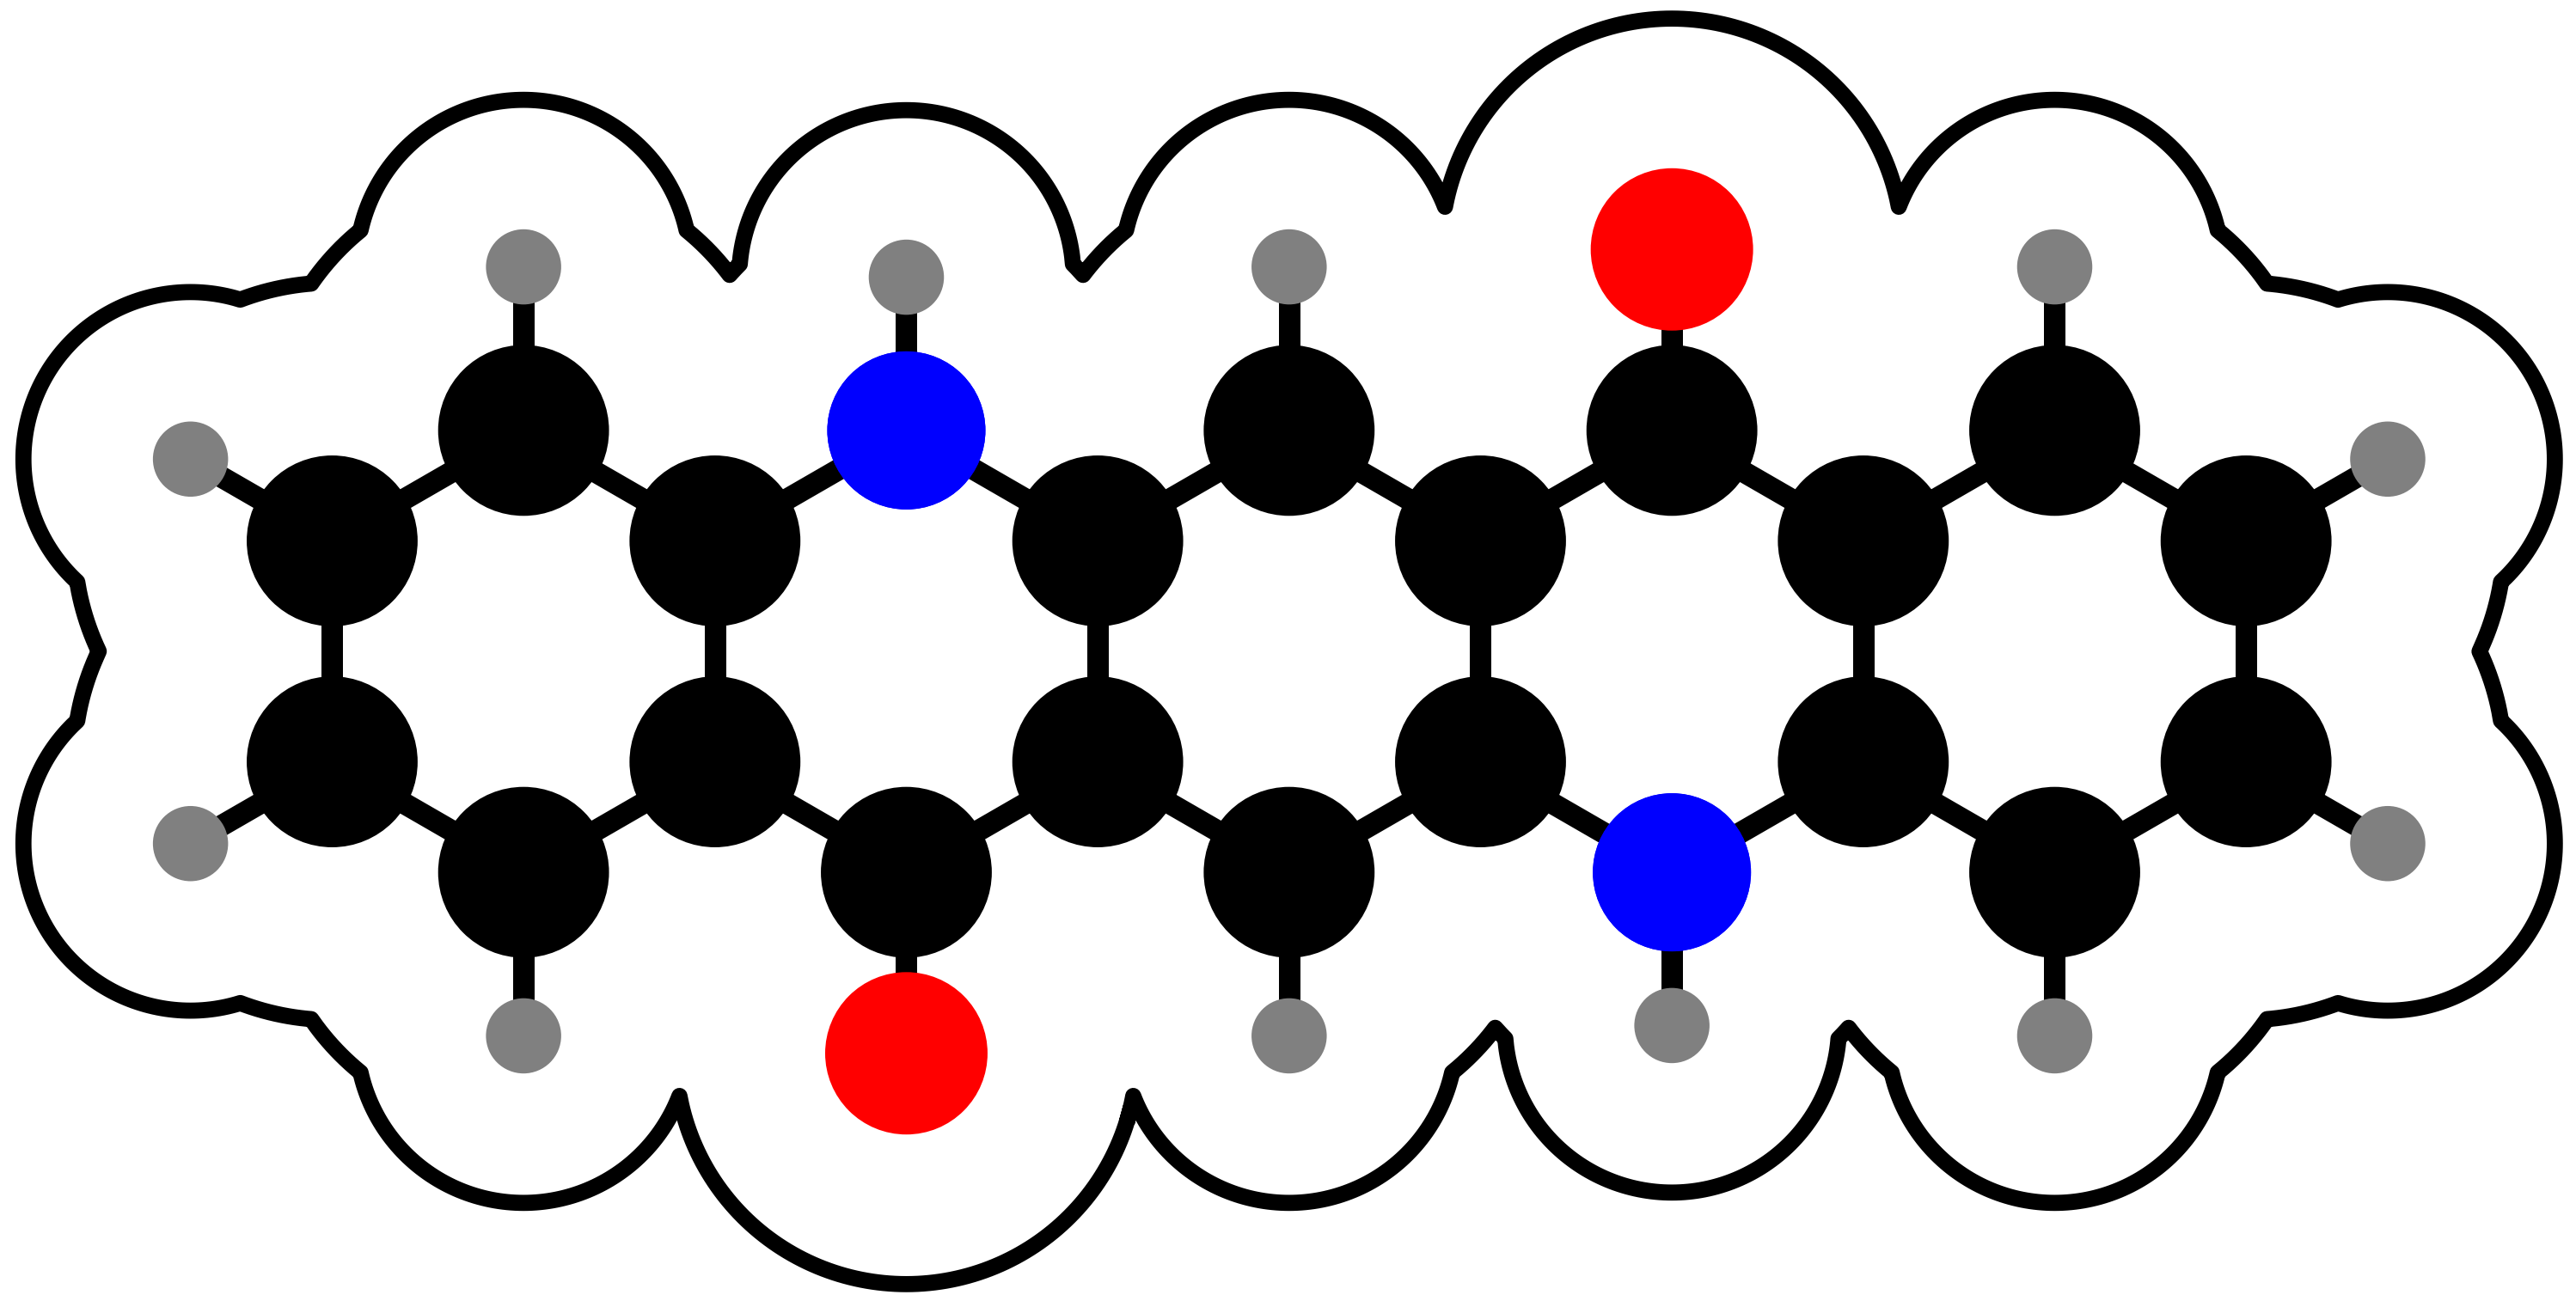
\includegraphics[width=\linewidth]{images/QA_molecule.png}
		\caption{Ball-and-stick model}
	\end{subfigure}
	\caption{Molecular structure of \acf{QA}.}
	\label{fig:QA}
\end{figure}


The molecule is classified as a heterocyclic compound. Its structure is characterized by a conjugated ring system that imparts significant rigidity and planarity to the molecule.\autocite{forBiotechnologyInformation2025}. \ac{QA} is of the symmetry group $\mathrm{C_{2h}}$ and has a molar mass of 312.32~\si{g/mol}. The molecule is a crystalline solid with four known different crystal structures under standard conditions.\autocite{Paulus2007,Mizuguchi}


\section{Structures of Quinachridone (QA) on the Ag(100) surface}

For \ac{QA} deposited onto the Ag(100) surface, two structural phases were observed to form: the $\alpha$- and $\beta$-phase. A thorough examination of these two phases has been conducted by N. Humberg.\autocite{Humberg2024, Humberg2020}

The formation of the $\alpha$-phase occurs subsequent to the deposition of the \ac{QA} molecules onto the Ag(100) surface at a sample temperature of 300~\si{K}. This phase is composed of parallel molecular chains that are flat-lying with the $\pi$-system being oriented parallel to the Ag(100) surface. The \ac{QA} molecules are connected via intermolecular hydrogen bonds between the keto groups of one molecular chain and the amine groups of another, resulting in 2 hydrogen bonds per molecule. It was also determined that the domains under consideration are homochiral, a finding that suggests a high degree of mobility for the \ac{QA} molecules on Ag(100) surface at 300~\si{K}.

In addition, the superstructure matrix of the $\alpha$-phase for a complete \ac{ML} was determined using a \ac{SPA-LEED} image and \ac{STM} results. The following superstructure matrix was found
\begin{equation*}
\mathbf{M_\alpha} =\begin{pmatrix}
2 & 1.25 \\
-3 & 4.80 
\end{pmatrix},
\end{equation*}
which shows that the structure is of the \ac{POL} type. This means that every lattice point of the superstructure falls on a substrate lattice line of the [10] direction of the Ag(100) surface. It should be noted that the intermolecular distance $b_1$ between the molecules of a chain are determined by the intermolecular hydrogen bonds and does not change with the coverage. The distance between two molecular chains $b_2$ increases with decreasing coverage.

The \ac{STM} images, the \ac{SPA-LEED} image and the structure model of \ac{QA} on Ag(100) in the $\alpha$-phase is illustrated in \autoref{fig:literature_alpha}.
\begin{figure}[htb]
	\centering
	\includegraphics[width=0.7\textwidth]{images/literature_alpha.png}
	\caption{Structure of complete \ac{ML} of \ac{QA} on Ag(100) in the $\alpha$-phase. The image shows an overview \ac{STM} image (a), a close-up \ac{STM} image of the molecular arrangement (b), the \ac{SPA-LEED} image (c) and the structure model (d). The image is taken from reference \cite{Humberg2024}.}
	\label{fig:literature_alpha}
\end{figure}
The phase transition from the $\alpha$-phase to the $\beta$-phase occurs when the sample is heated up to 500~\si{K} for 15 minutes. The phase transition is irreversible. This means that the $\alpha$-phase is metastable and is stabilized by a kinetic barrier. This kinetic barrier corresponds to the energy required to break the hydrogen bonds between the \ac{QA} molecules in the $\alpha$-phase.

For the $\beta$-phase, the investigation revealed a 2D network of molecular chains, which are comprised of dimers and manifest periodic indents. The existing structure model proposes a single hydrogen bond between the dimers instead of theoretical two possible hydrogen bonds. The two molecules of the dimer form two hydrogen bonds with each other, resulting in 1.5 hydrogen bonds per molecule.

Once more, employing a \ac{SPA-LEED} image and \ac{STM} results, the superstructure matrix of the $\beta$-phase for a complete \ac{ML} was determined as
\begin{equation*}
\mathbf{M_\beta} =\begin{pmatrix}
4 & 3 \\
-5 & 3 
\end{pmatrix},
\end{equation*}
which means that the structure is commensurate. In comparison to the \ac{POL} type of the $\alpha$-phase, the commensurate structure of the $\beta$-phase indicates that the superstructure for the $\beta$-phase is aligned with the substrate in a way that the periodicity of the superstructure is a multiple of the substrate lattice constant. In general, the commensurate structure of the $\beta$-phase indicates a stronger interaction with the substrate and relates to energy gain compared to the $\alpha$-phase.\autocite{Hooks2001}

The \ac{STM} images, the \ac{SPA-LEED} image and the structure model of \ac{QA} on Ag(100) in the $\beta$-phase is illustrated in \autoref{fig:literature_beta}.
\begin{figure}[htb]
	\centering
	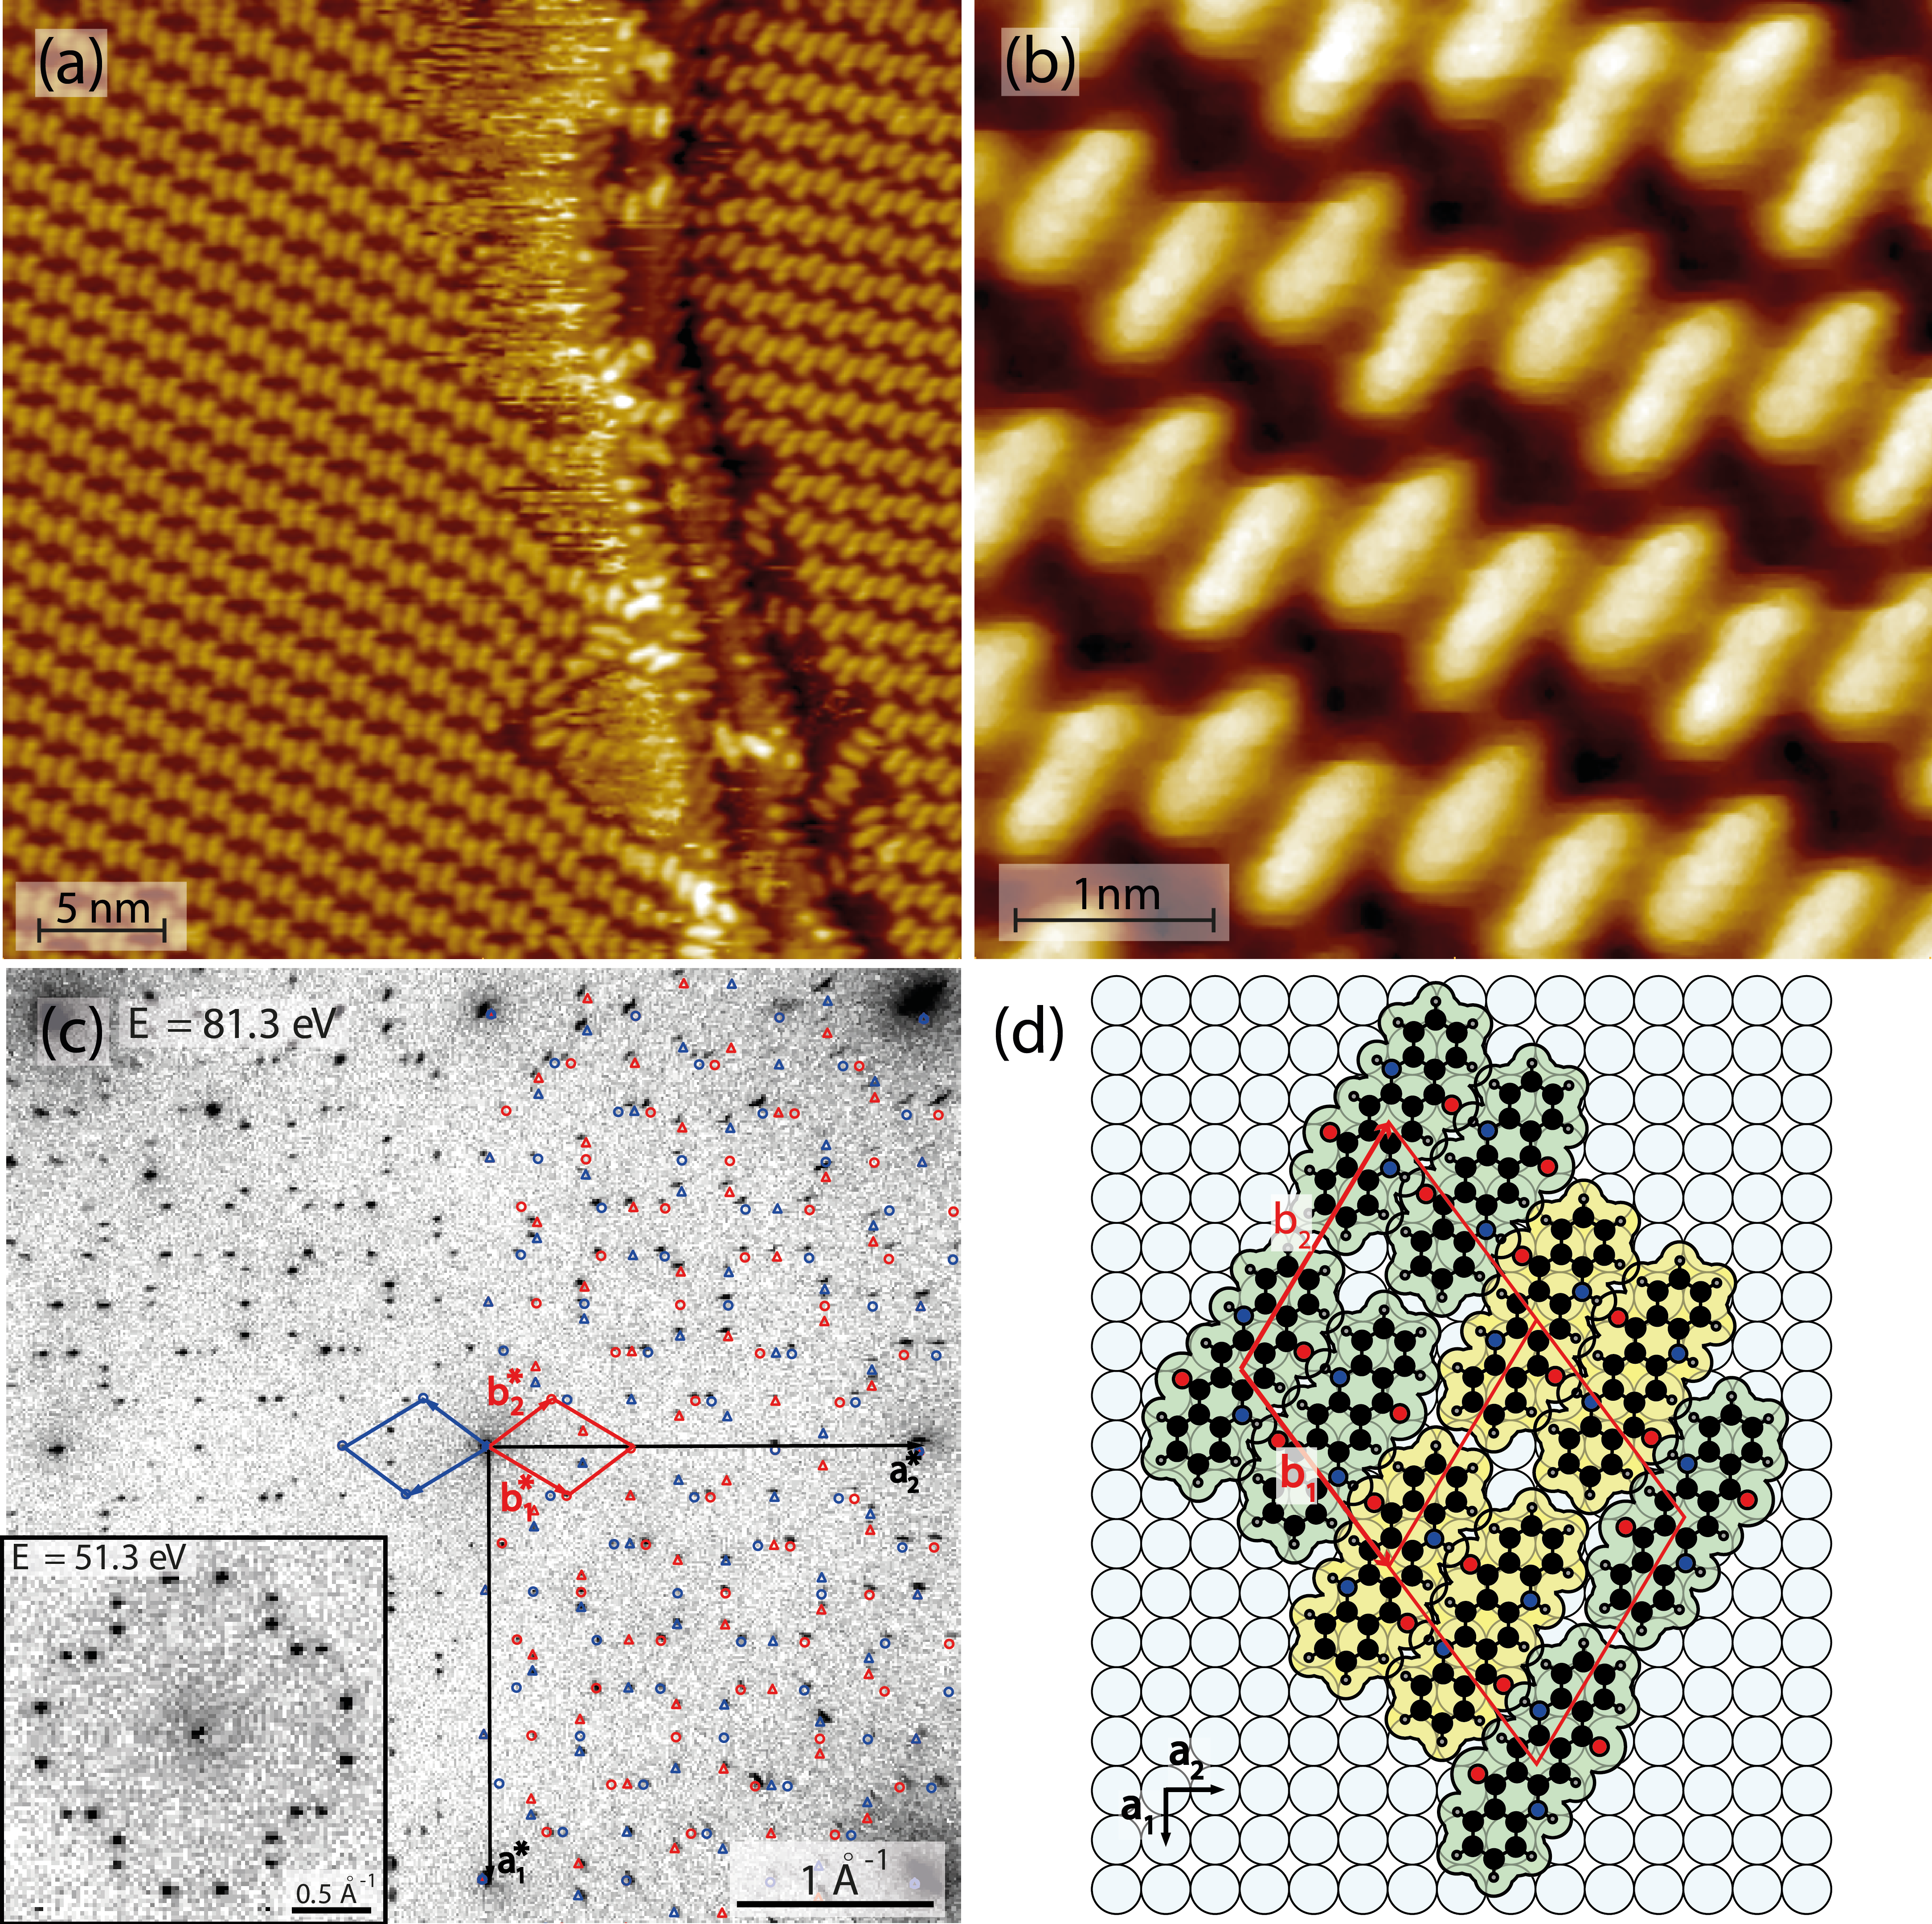
\includegraphics[width=0.7\textwidth]{images/literature_beta.png}
	\caption{Structure of complete \ac{ML} of \ac{QA} on Ag(100) in the $\beta$-phase. The image shows an overview \ac{STM} image (a), a close-up \ac{STM} image of the molecular arrangement (b), the \ac{SPA-LEED} image (c) and the structure model (d). The image is taken from reference \cite{Humberg2024}.}
	\label{fig:literature_beta}
\end{figure}
\cleardoublepage